\documentclass[a4paper, 11pt]{article}

%-------------------------------------------------------------------------------
%--- (a) Required Packages
%-------------------------------------------------------------------------------
\usepackage{amsmath,amsfonts,amssymb,amsthm}
\usepackage{adjustbox}
\usepackage{mwe}
\usepackage{authblk}
\usepackage[english]{babel}
\usepackage[para,online,flushleft]{threeparttable}
\usepackage{lscape}
\usepackage{threeparttablex}
\usepackage{tabu}
\usepackage{booktabs}
\usepackage{caption}
\usepackage{subcaption}
\usepackage[usenames, dvipsnames]{color}
\usepackage{epstopdf}
\usepackage[capposition=top]{floatrow}
\usepackage{framed}
%\usepackage[T1]{fontenc}
\usepackage{lmodern}
\usepackage{graphicx}
\usepackage{hyperref}
\usepackage[utf8]{inputenc}
\usepackage{lscape}
\usepackage{multirow}
\usepackage{natbib}
\usepackage{setspace}
\usepackage{rotating}
\usepackage{subcaption}
\usepackage{subfloat}
\usepackage{url}
\usepackage{wrapfig}
\usepackage{multicol}
\usepackage[toc,page]{appendix}
\usepackage{float}
\interfootnotelinepenalty=10000
\usepackage[a4paper]{geometry}
\usepackage{textcomp}
\usepackage{longtable}
\usepackage{babel,blindtext}
%-------------------------------------------------------------------------------
%--- (b) Specific margins
%-------------------------------------------------------------------------------
\setlength  \textwidth{\paperwidth}
\setlength  \textheight{\paperheight}
\setlength  \oddsidemargin{3cm}
\setlength  \topmargin{-1.2cm}
\setlength  \footnotesep{2ex}
\addtolength\textheight{-6cm}
\addtolength\textwidth{-6cm}
\addtolength\oddsidemargin{-1in}
 
%%ADDED SPACE BETWEEN PARAGRAPHS 
%-------------------------------------------------------------------------------
%--- (c) Internal Ref stype
%-------------------------------------------------------------------------------

\hypersetup{
    colorlinks=true,   
    linkcolor=Black,
    citecolor=BlueViolet,
    filecolor=BlueViolet,
    urlcolor=Black
}

 
%-------------------------------------------------------------------------------
%---  ABSTACT
%-------------------------------------------------------------------------------
\renewcommand\thesection{\Alph{section}}
\renewcommand*{\thepage}{A\arabic{page}}



\renewcommand{\thetable}{A\arabic{table}}
\renewcommand{\thefigure}{A\arabic{figure}}
\setcounter{page}{0}

\begin{document}
\begin{spacing}{1.4}
  \begin{center}
    \textbf{ONLINE APPENDIX} \\
    \vspace{4mm}
    For the paper: \\
    \vspace{6mm}
           {\large \textsc{The impact of abortion legalization on fertility and maternal
               mortality: New evidence from Mexico}} \\
    \vspace{3mm}
    Damian Clarke and Hanna M\"uhlrad
\end{center}

\tableofcontents
\setlength\parindent{0.25in}
\setlength\parskip{0.25in}

\newpage

%%%%%%%%%%%%%%%%%%%%%%%%%%%%%%%%%%%%%%%%%%%%%%%%%%%%%%%%%%%%%%%%%%%%%%%%%%%%%%%%%%%%%%%%
%%%%%%%%% Data Appendix 
\section{Data Appendix-MxFLS}\label{mxfls}
 
 
 In order to examine potential mechanisms through which the reform may have affected fertility and maternal mortality, we use longitudinal data on contraceptive use and knowledge from the Mexican Family Life Survey (MxFLS). The MxFLS is a nationally representative longitudinal dataset that follows individuals over time, covering various topics regarding the well-being of the Mexican population including information on reproductive health. This survey was conducted during three waves in 2002-2003, 2005-2006 and 2009-2012. The data between the years when the survey was conducted is generated by linear interpolation. The sample used for our analysis consists of women aged 15-44 who completed the reproductive health questionnaire resulting in a total of 15,114 individuals. Table~\ref{MXFLS} in the appendix presents descriptive statistics. Modern contraceptives are condoms, oral or/injectable/implants of hormones preventing ovulation, IUD, sterilization and emergency contraception. Traditional or less safe methods are calendar method or rhythm method, coitus interrupts, herbs or teas. For a detailed account of modern and traditional methods, see for instance WHO: \url{http://www.who.int/mediacentre/factsheets/fs351/en/}.
 
 
 
 %%%%% MxFLS Table     %%%%%%%%%%%%%%%%%%%%%%%%%%%%%%%%%%%%%%%%%%%%%%%%%%%%%%%%%%%%%%%%%
 
  \renewcommand{\thetable}{A\arabic{table}}
  \setcounter{table}{0}
    \renewcommand{\thefigure}{A\arabic{table}}
    \setcounter{figure}{0}
 \begin{table}[H]\caption{Descriptives MxFLS data}\label{MXFLS}
 	
 	\begin{threeparttable}
 		
 {\footnotesize  		

\begin{tabular}{lcccccc}
	\hline\hline
	&		&		&		&		&		&	 	\\
	\multirow{1}{*}{} &
	\multicolumn{3}{c}{Mexico City}&\multicolumn{3}{c}{The rest of Mexico}\\ \cmidrule(r){2-4} \cmidrule(l){5-7}


Variable	&	Mean	&	Std.	&	Obs	&	Mean	&	Std.	&	Obs	\\\hline


Contraception use	&	0,647	&	0,479	&	0,479	&	0,604	&	0,489	&	14766	\\
Modern Contraception use	&	0,612	&	0,488	&	0,488	&	0,563	&	0,496	&	14768	\\
Knowledge of contraception	&	0,981	&	0,137	&	0,137	&	0,969	&	0,173	&	23473	\\





\hline\hline
\end{tabular}}
 		{\scriptsize 	
 			\begin{tablenotes}
 				
 				\item Note to Table~\ref{MXFLS}: The data is obtained from the Mexican Family Life Survey (MxFLS).   
 			\end{tablenotes}}
 			
 		\end{threeparttable}
 		
 	\end{table}
   \begin{figure}[H]
   	
   	\centering	\caption{MxFLS data}
   	
   	\label{MxFLS_Graphs}
   	
   	\begin{subfigure}{.3\textwidth}
   		\centering	\caption{Current use of modern method}\label{modmethod}
   		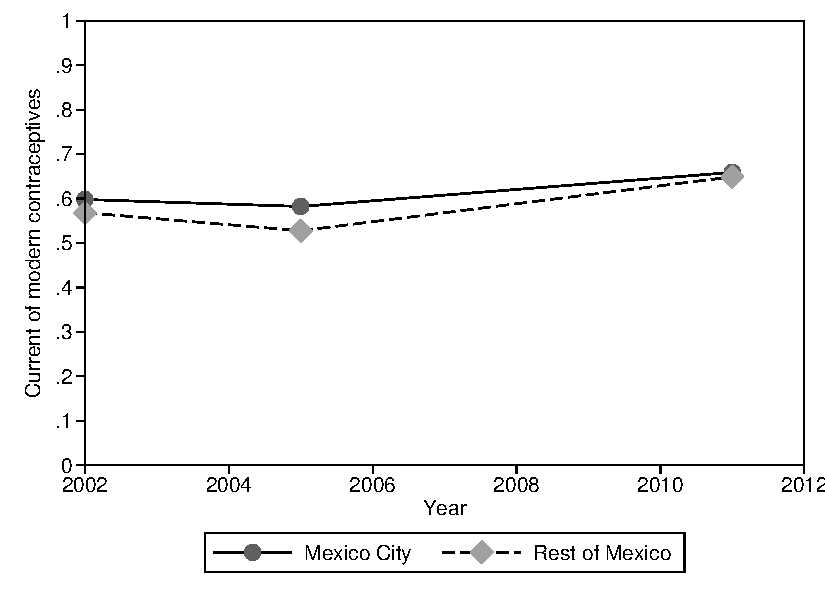
\includegraphics[scale=0.3]{figures/Trend_ModMethod.pdf}
   	\end{subfigure}%
   	\begin{subfigure}{.3\textwidth}
   		\centering\caption{Current use of modern or traditional method}\label{anymethod}
   		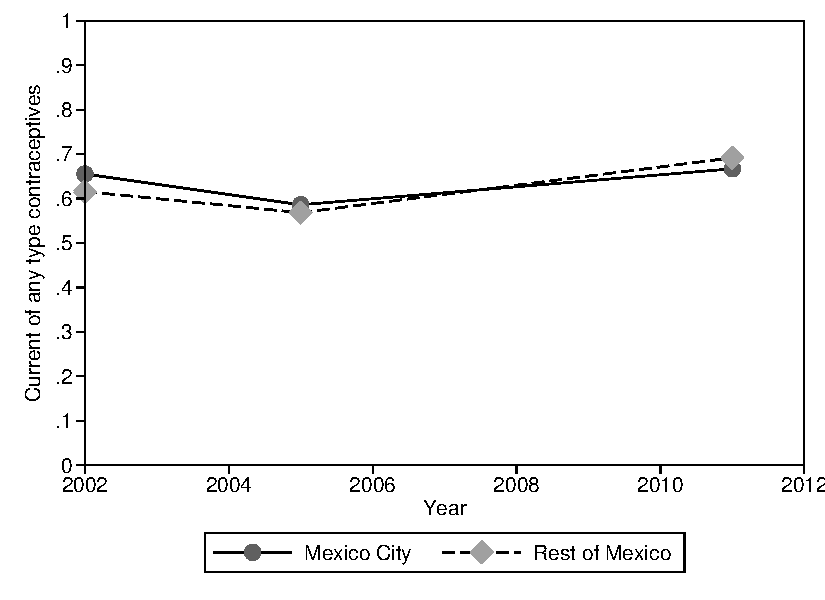
\includegraphics[scale=0.3]{figures/Trend_AnyMethod.pdf}
   	\end{subfigure}%
   	\begin{subfigure}{.3\textwidth}
   		\centering	\caption{Contraceptive knowledge}	\label{knowledge}
   		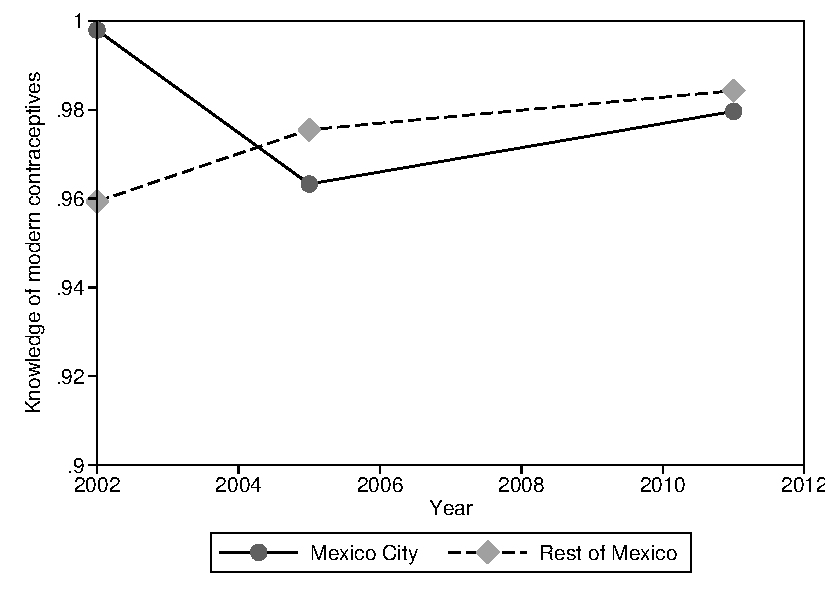
\includegraphics[scale=0.3]{figures/Trend_ContraKnow.pdf}
   	\end{subfigure}
   	
   	
{\footnotesize    	\floatfoot{Note to Figure~\ref{MxFLS_Graphs}: The data is obtained from the Mexican Family Life Survey (MxFLS) conducted in 2002-2003, 2005-2006 and 2009-2012. The sample consists of all women aged 15-44 who completed the reproductive health questionnaire resulting in a total of 15,114 individuals. The data for the years between when the surveys were conducted is linearly interpolated. Modern contraceptives are condoms, oral or/injectable/implants of hormones preventing ovulation, IUD, sterilization and emergency contraception. Traditional or less safe methods are calendar method or rhythm method, coitus interrupts, herbs or teas. }}
   	
   \end{figure}
% Data on contraceptive use and knowledge among adult and teenage women are obtained from the Mexico National Health Survey (ENSA) conducted in 2000 and the Mexican National Survey of Health and Nutrition (ENSANUT) conducted in 2006 and 2012. This data is a nationally representative household survey of repeated cross sections, covering various topics regarding nutrition and health, including information on reproductive health. This survey was conducted in 2000, 2006 and 2012 and covers 45,870, 48,304 and 50,000 households per wave respectively. The data between the years when the survey was conducted is generated by linear interpolation. The sample used for constructing the state level contraceptive control variables, consists of women aged 15-44 who completed the reproductive health questionnaire.
 
 
 
 \section{Tables}
 \renewcommand{\thetable}{B\arabic{table}}
\setcounter{table}{0}
%%%%%%%%%%%%%%%%%%%%%%%%%%%%%%%%%%%%%%%%%%%%%%%%%%%%%%%%%%%%%%%%%%%%%%%%%%%%%%%%%%%%%%%
%%%%% List of States %%%%%%%%%%%%%%%%%%%%%%%%%%%%%%%%%%%%%%%%%%%%%%%%%%%%%%%%%%%%%%%%%% 
 
\begin{table}[H]\caption{List of States}\label{list_of_states}
		\begin{threeparttable}
	

\begin{tabular}{lcc}
	\hline\hline
&&\\
	\multirow{1}{*}{State} &
	\multicolumn{1}{c}{\shortstack{Number of \\ maternal deaths}}&\multicolumn{1}{c}{\shortstack{Number of \\ births}}\\ &&\\   \hline
 
Aguascalientes	&	87	&	257,576	\\
Baja California	&	250	&	5,68,276	\\
Baja California Sur	&	53	&	120,621	\\
Campeche	&	88	&	160,185	\\
Chiapas	&	825	&	1,220,254	\\
Chihuahua	&	440	&	678,600	\\
Coahuila	&	198	&	552,608	\\
Colima	&	31	&	120,840	\\
Distrito Federal (Mexico City)	&	818	&	1,505,790	\\
Durango	&	154	&	362,410	\\
Guanajuato	&	489	&	1,160,802	\\
Guerrero	&	702	&	809,783	\\
Hidalgo	&	297	&	538,216	\\
Jalisco	&	577	&	1,522,825	\\
State of México	&	1,745	&	3,186,751	\\
Michoacán	&	458	&	946,165	\\
Morelos	&	185	&	326,129	\\
Nayarit	&	109	&	216,272	\\
Nuevo León	&	204	&	882,618	\\
Oaxaca	&	639	&	851,138	\\
Puebla	&	739	&	1,377,091	\\
Querétaro	&	168	&	385,391	\\
Quintana Roo	&	136	&	256,223	\\
San Luis Potosí	&	276	&	552,094	\\
Sinaloa	&	173	&	554,838	\\
Sonora	&	197	&	513,172	\\
Tabasco	&	211	&	477,473	\\
Tamaulipas	&	258	&	630,260	\\
Tlaxcala	&	121	&	261,363	\\
Veracruz	&	922	&	1,467,936	\\
Yucatán	&	176	&	360,051	\\
Zacatecas	&	132	&	333,368	\\ 
 \hline\hline
\end{tabular}
{\footnotesize 	\begin{tablenotes}
	\item Administrative data made available by INEGI on all births and maternal deaths by each state for ages 15-44 during the time period 2002-2011.
\end{tablenotes}}
\end{threeparttable}
\end{table}

%%%%%%%%%%%%%%%%%%%%%%%%%%%%%%%%%%%%%%%%%%%%%%%%%%%%%%%%%%%%%%%%%%%%%%%%%%%%%%%%%%%%%%%
%%%%% EXPOSURE %%%%%%%%%%%%%%%%%%%%%%%%%%%%%%%%%%%%%%%%%%%%%%%%%%%%%%%%%%%%%%%%%%%%%%%% 

\begin{sidewaystable}[H] \caption{Exposure to the reform at time of conception}\label{Exposure}

\centering   \begin{threeparttable}  {\small \begin{tabular}{lccccccccc}
 \hline\hline   \multirow{1}{*}{} &
 \multicolumn{3}{c}{\textbf{Fertility}} & 	\multicolumn{3}{c}{\textbf{Maternal Mortality}} \\\cline{2-4}\cline{5-7} 
 
  \multirow{2}{*}{} &&
		
		\multicolumn{1}{c}{\textbf{Partial exposure}} & 	\multicolumn{1}{c}{\textbf{Full exposure}}&&\multicolumn{1}{c}{\textbf{Partial exposure}} & 	\multicolumn{1}{c}{\textbf{Full exposure}}\\ 
		
	 
		\textit{Month of}   & \textit{Month of}  & \textit{Abortion legal at}   & \textit{Abortion legal at}  & \textit{Month of}  & \textit{Spillover effect}   & \textit{No spillover effects}\\ 
		
		\textit{Conception}& \textit{Birth}&\textit{at the month}&\textit{some point during} & \textit{Death}&\textit{from illegal  }&\textit{and abortion}\\
		
	 &  &\textit{of conception}&\textit{the first trimester} & &\textit{abortions}&\textit{available the full}\\
		&  & & &  & &\textit{1st trimester}\\
		\hline 
 

24 Dec 06-23 Jan 07	&	24 Sep-23 Oct, 2007	&	no	&	no	&	24 Apr-23 May, 2007	&	yes 	&	no	\\
24 Jan-23 Feb, 2007	&	24 Oct-23 Nov, 2007	&	yes	&	no	&	24 May-23 Jun, 2007	&	yes 	&	no	\\
24 Feb-23 Mar, 2007	&	24 Nov-23 Dec, 2007	&	yes	&	no	&	24 Jun-23 Jul, 2007	&	yes 	&	no	\\
24 Mar-23 Apr, 2007	&	24 Dec 07-23 Jan, 08	&	yes	&	no	&	24 Jul-23 Aug, 2007	&	yes 	&	no	\\
24 Apr-23 May, 2007	&	24 Jan-23 Feb, 2008	&	-	&	yes	&	24 Aug-23 Sep, 2007	&	yes 	&	no	\\
24 May-23 Jun, 2007	&	24 Feb-23 Mar, 2008	&	-	&	yes	&	24 Sep-23 Oct, 2007	&	yes 	&	no	\\
24 Jun-23 Jul, 2007	&	24 Mar-23 Apr, 2008	&	-	&	yes	&	24 Oct-23 Nov, 2007	&	no	&	yes	\\
24 Jul-23 Aug, 2007	&	24 Apr-23 May, 2008	&	-	&	yes	&	24 Nov-23 Dec, 2007	&	-	&	yes	\\
24 Aug-23 Sep, 2007	&	24 May-23 Jun, 2008	&	-	&	yes	&	24 Dec 07-23 Feb 08	&	-	&	yes	\\
24 Sep-23 Oct, 2007	&	24 Jun-23 Jul, 2008	&	-	&	yes	&	24 Jan-23 Feb, 2008	&	-	&	yes	\\


\hline 	\hline 


 \end{tabular} }

  		\begin{tablenotes}

  			\small

  			The table displays exposure to the reform at time of conception for birth and maternal deaths respectively. The abortion law was passed on 24 April 2007. In terms of fertility outcome, the full effect of the reform will be observed in January 2008 since fertility exhibits a nine month lag due to realization of gestation (assuming 40 weeks of gestation). That is, women who got pregnant after the law was passed, had access to abortion during their whole first trimester and are therefore considered as fully treated. Women who got pregnant 3 months before the law was passed, had at least some period of time when they could access the reform, and are therefore considered partially treated. The earliest time for which any impact on fertility can be detected would then be from October 2007 and onwards. Regarding maternal mortality, women conceiving after 24 January 2007 could access the reform at least some point during the first trimester while women conceiving after the reform was passed could access the reform during the whole first trimester. However, women conceiving before 24 January 2007, that is women pregnant beyond their first trimester at the time when the reform was passed, could have an illegal abortion during the remaining 6 months of their pregnancy and hence ``contaminate'' the maternal deaths taking place in the 6 months after the reform was passed. The fully exposed maternal deaths (without contamination) therefore occurs from 24 October and forward. Additionally, we also expect a lagged effect from maternal mortality since it is a function of fertility (i.e lower fertility implies lower mortality).  
  			
  			           

  		\end{tablenotes}

  \end{threeparttable} 	

\end{sidewaystable}  
 
%%%%%%%%%%%%%%%%%%%%%%%%%%%%%%%%%%%%%%%%%%%%%%%%%%%%%%%%%%%%%%%%%%%%%%%%%%%%%%%%%%%%%%%
%%%%% Trend REG %%%%%%%%%%%%%%%%%%%%%%%%%%%%%%%%%%%%%%%%%%%%%%%%%%%%%%%%%%%%%%%%%%%%%%% 

\begin{table}[H]\caption{Test for parallel trends in the outcome variables in the pre-treatment period}\label{trendreg}  
	\begin{threeparttable}	
	{
\def\sym#1{\ifmmode^{#1}\else\(^{#1}\)\fi}
\begin{tabular}{l*{2}{c}}
\hline\hline
                    &\multicolumn{1}{c}{(1)}&\multicolumn{1}{c}{(2)}\\
                    &\multicolumn{1}{c}{\shortstack{OLS\\ Log N. Births}}&\multicolumn{1}{c}{\shortstack{Poisson\\ N. Deaths}}\\
\hline
                 &               &               \\
Control Area=1 $\times$ Trend&    0.000236   &    -0.00147   \\
                    &     (0.065)   &     (0.043)   \\
[1em]
Trend               &    -0.00788   &     -0.0187   \\
                    &     (0.063)   &     (0.041)   \\
[1em]
Control Area=1      &      -1.641   &       1.974   \\
                    &   (129.402)   &    (86.760)   \\
\hline
Observations        &        4650   &        4650   \\
\(R^{2}\)           &     0.02446   &               \\
Pseudo \(R^{2}\)    &               &     0.01965   \\
\hline\hline
\end{tabular}
}

{\footnotesize 	\begin{tablenotes}
	\item The table displays OLS regression (column 1) and Poisson regression (column2). A linear time trend is interacted with the control group (Trend $*$ Control Area) for the pre-treatment period 2002-2006. Robust standard errors in brackets.*** p$<$0.01,** p$<$0.05,* p$<$0.1
\end{tablenotes}}
\end{threeparttable}
\end{table}

%%%%%%%%%%%%%%%%%%%%%%%%%%%%%%%%%%%%%%%%%%%%%%%%%%%%%%%%%%%%%%%%%%%%%%%%%%%%%%%%%%%%%%%
%%%%% MxFLS Table     %%%%%%%%%%%%%%%%%%%%%%%%%%%%%%%%%%%%%%%%%%%%%%%%%%%%%%%%%%%%%%%%%
 

 
%%%%%%%%%%%%%%%%%%%%%%%%%%%%%%%%%%%%%%%%%%%%%%%%%%%%%%%%%%%%%%%%%%%%%%%%%%%%%%%%%%%%%%%
%%%%% Monthly Results %%%%%%%%%%%%%%%%%%%%%%%%%%%%%%%%%%%%%%%%%%%%%%%%%%%%%%%%%%%%%%%%%

\begin{sidewaystable}[H]\caption{The Effect of the Reform on Births, monthly data} \label{BirthMonth}
	
	\begin{threeparttable}
		
		{\footnotesize  {
\def\sym#1{\ifmmode^{#1}\else\(^{#1}\)\fi}
\begin{tabular}{l*{10}{c}}
\hline\hline
                    &\multicolumn{5}{c}{\textbf{Full-Sample 15-44}}                                 &\multicolumn{5}{c}{\textbf{Teenage women 15-19}}                               \\\cmidrule(lr){2-6}\cmidrule(lr){7-11}
                    &\multicolumn{1}{c}{(1)}&\multicolumn{1}{c}{(2)}&\multicolumn{1}{c}{(3)}&\multicolumn{1}{c}{(4)}&\multicolumn{1}{c}{(5)}&\multicolumn{1}{c}{(6)}&\multicolumn{1}{c}{(7)}&\multicolumn{1}{c}{(8)}&\multicolumn{1}{c}{(9)}&\multicolumn{1}{c}{(10)}\\
                    &\multicolumn{1}{c}{\shortstack{OLS\\Log\\ Num. of \\Births}}&\multicolumn{1}{c}{\shortstack{OLS\\Log \\Num. of \\Births}}&\multicolumn{1}{c}{\shortstack{OLS\\Log\\ Num. of \\Births}}&\multicolumn{1}{c}{\shortstack{OLS\\Log \\Num. of \\Births}}&\multicolumn{1}{c}{\shortstack{OLS\\Log\\ Num. of \\Births}}&\multicolumn{1}{c}{\shortstack{OLS\\Log\\ Num. of \\Births}}&\multicolumn{1}{c}{\shortstack{OLS\\Log \\Num. of \\Births}}&\multicolumn{1}{c}{\shortstack{OLS\\Log\\ Num. of \\Births}}&\multicolumn{1}{c}{\shortstack{OLS\\Log \\Num. of \\Births}}&\multicolumn{1}{c}{\shortstack{OLS\\Log\\ Num. of \\Births}}\\
\hline
PartiallyBirth      &     -0.0217*  &    -0.00821   &    -0.00692   &     -0.0101   &    -0.00919   &     -0.0153   &    -0.00489   &    -0.00284   &    -0.00526   &   -0.000861   \\
                    &     (0.013)   &     (0.009)   &     (0.009)   &     (0.011)   &     (0.011)   &     (0.014)   &     (0.011)   &     (0.010)   &     (0.011)   &     (0.012)   \\
[1em]
FullyBirth          &     -0.0307***&    -0.00781   &     -0.0166***&     -0.0147** &     -0.0144** &     -0.0551***&     -0.0375***&     -0.0517***&     -0.0461***&     -0.0467***\\
                    &     (0.011)   &     (0.005)   &     (0.006)   &     (0.006)   &     (0.006)   &     (0.011)   &     (0.007)   &     (0.008)   &     (0.009)   &     (0.008)   \\
\hline
\(R^{2}\)           &       0.970   &       0.970   &       0.970   &       0.970   &       0.970   &       0.977   &       0.978   &       0.978   &       0.978   &       0.978   \\
Mean\_of\_dep\_Var     &       4.562   &       4.562   &       4.562   &       4.562   &       4.562   &       4.846   &       4.846   &       4.846   &       4.846   &       4.846   \\
Observations (State*Year*Age) & 111529&111529& 111529&111529&111529&18653&18653&18653&18653&18653\\
\hline State, Year and Age FE& \checkmark &\checkmark&\checkmark& \checkmark&\checkmark&\checkmark&\checkmark&\checkmark&\checkmark&\checkmark\\
State Specific Linear Trends&&\checkmark&\checkmark&\checkmark&\checkmark&& \checkmark&\checkmark&\checkmark&\checkmark\\
Economic controls&& &\checkmark& \checkmark&\checkmark&&&\checkmark&\checkmark&\checkmark\\
Education controls&&&& \checkmark&\checkmark&&&&\checkmark&\checkmark\\
Health controls&&&&& \checkmark&&&&&\checkmark\\\bottomrule\bottomrule
\end{tabular}}
}
		
		\begin{tablenotes}
			
			\footnotesize
			
			\item \textit{Notes to Table~\ref{BirthMonth}}. The table displays the difference in difference estimates from OLS regressions. The sample consists of all births among women aged 15-44 (column 1-5) and sub-sample of teenage women aged 15-19 (column 6-10), for the period 2002-2011, on a monthly level. Partially treated women (who had some exposure to the reform but not during the entire trimester), such that birth occurring between Oct-Dec 2007, are excluded from the sample. The dependent variables are defined as the log number of births. The independent variable \textit{Reform} takes the value 1 in Mexico City 9 months after the law was passed due to realization of gestation and 0 otherwise. Similarly, \textit{ReformClose} is a binary variable equal to 1 in the neighboring State of Mexico 9 months after the reform was introduced. The economic controls are state level income, unemployment and rurality. The educational controls are illiteracy and proportion of people aged 6-14 who are not enrolled in school. The health controls are the proportion of residents with no health rights and the roll out of the national health insurance program ``Seguro Popular''. The fixed effects consists of age, state and year binary variables. Standard errors are clustered at state level.*** p$<$0.01,** p$<$0.05,* p$<$0.1.
			 
			
		\end{tablenotes} 
		
	\end{threeparttable}
	
\end{sidewaystable}

\begin{sidewaystable}[H]\caption{The Effect of the Reform on Maternal Mortality, monthly data} \label{MMRMonth}
	
\begin{threeparttable}
		
{\footnotesize  {
\def\sym#1{\ifmmode^{#1}\else\(^{#1}\)\fi}
\begin{tabular}{l*{10}{c}}
\hline\hline
                    &\multicolumn{5}{c}{\textbf{Full-Sample 15-44}}                                 &\multicolumn{5}{c}{\textbf{Teenage women 15-19}}                               \\\cmidrule(lr){2-6}\cmidrule(lr){7-11}
                    &\multicolumn{1}{c}{(1)}&\multicolumn{1}{c}{(2)}&\multicolumn{1}{c}{(3)}&\multicolumn{1}{c}{(4)}&\multicolumn{1}{c}{(5)}&\multicolumn{1}{c}{(6)}&\multicolumn{1}{c}{(7)}&\multicolumn{1}{c}{(8)}&\multicolumn{1}{c}{(9)}&\multicolumn{1}{c}{(10)}\\
                    &\multicolumn{1}{c}{\shortstack{Poisson\\\\Num. \\Maternal \\Deaths}}&\multicolumn{1}{c}{\shortstack{Poisson\\\\Num. \\Maternal \\Deaths}}&\multicolumn{1}{c}{\shortstack{Poisson\\\\Num. \\Maternal \\Deaths}}&\multicolumn{1}{c}{\shortstack{Poisson\\\\Num. \\Maternal \\Deaths}}&\multicolumn{1}{c}{\shortstack{Poisson\\\\Num. \\Maternal \\Deaths}}&\multicolumn{1}{c}{\shortstack{Poisson\\\\Num. \\Maternal \\Deaths}}&\multicolumn{1}{c}{\shortstack{Poisson\\\\Num. \\Maternal \\Deaths}}&\multicolumn{1}{c}{\shortstack{Poisson\\\\Num. \\Maternal \\Deaths}}&\multicolumn{1}{c}{\shortstack{Poisson\\\\Num. \\Maternal \\Deaths}}&\multicolumn{1}{c}{\shortstack{Poisson\\\\Num. \\Maternal \\Deaths}}\\
\hline

PartiallyMMR        &      0.0947*  &      0.0744   &      0.0562   &      0.0608   &      0.0634   &       0.306*  &       0.230   &       0.229   &       0.211   &       0.212   \\
                    &     (0.052)   &     (0.066)   &     (0.065)   &     (0.064)   &     (0.066)   &     (0.179)   &     (0.172)   &     (0.176)   &     (0.174)   &     (0.175)   \\
[1em]
FullyMMR            &     -0.0414   &     -0.0728   &      -0.102** &     -0.0776*  &     -0.0809*  &     -0.0966   &      -0.212** &      -0.231** &      -0.331** &      -0.312*  \\
                    &     (0.026)   &     (0.049)   &     (0.048)   &     (0.046)   &     (0.045)   &     (0.061)   &     (0.089)   &     (0.100)   &     (0.147)   &     (0.169)   \\
\hline
Pseudo \(R^{2}\)    &     0.13641   &     0.13712   &     0.13725   &     0.13726   &     0.13726   &     0.14010   &     0.14307   &     0.14309   &     0.14325   &     0.14365   \\
Mean\_of\_dep\_Var     &       0.103   &       0.103   &       0.103   &       0.103   &       0.103   &      0.0785   &      0.0785   &      0.0785   &      0.0785   &      0.0785   \\
Observations (State*Year*Age) & 115146&115146& 115146&115146&115146&19259&19259&19259&19259&19259\\
\hline State, Year and Age FE& \checkmark &\checkmark&\checkmark& \checkmark&\checkmark&\checkmark&\checkmark&\checkmark&\checkmark&\checkmark\\
State Specific Linear Trends&&\checkmark&\checkmark&\checkmark&\checkmark&& \checkmark&\checkmark&\checkmark&\checkmark\\
Economic controls&& &\checkmark& \checkmark&\checkmark&&&\checkmark&\checkmark&\checkmark\\
Education controls&&&& \checkmark&\checkmark&&&&\checkmark&\checkmark\\
Health controls&&&&& \checkmark&&&&&\checkmark\\\bottomrule\bottomrule
\end{tabular}}
}
		
\begin{tablenotes}
			
\footnotesize
			
\item \textit{Notes to Table~\ref{MMRMonth}}. The table displays the difference in difference estimates from OLS regressions. The sample consists of all maternal deaths among women aged 15-44 (column 1-5) and sub-sample of teenage women aged 15-19 (column 6-10), for the period 2002-2011, on a monthly level. Partially treated maternal deaths are deaths occurring between April-October 2007 because these deaths could be due to induced abortion beyond the first trimester, which would not occur if these women have had access to legal first trimester abortion. These are excluded from the sample. The dependent variables are defined as the number of maternal deaths. The independent variable \textit{Reform} takes the value one in Mexico City 6 months after the law was passed on order to account for late term abortions. Similarly, \textit{ReformClose} is a binary variable equal to one in the neighboring State of Mexico 6 months after the reform was introduced. The economic controls are state level income, unemployment and rurality. The educational controls are illiteracy and proportion of people aged 6-14 who are not enrolled in school. The health controls are the proportion of residents with no health rights and the roll out of the national health insurance program ``Seguro Popular''. The fixed effects consists of age, state and year binary variables. Standard errors are clustered at state level.*** p$<$0.01,** p$<$0.05,* p$<$0.1.
 
			
\end{tablenotes} 
		
\end{threeparttable}
	
\end{sidewaystable}

%%%%%%%%%%%%%%%%%%%%%%%%%%%%%%%%%%%%%%%%%%%%%%%%%%%%%%%%%%%%%%%%%%%%%%%%%%%%%%%%%%%%%%%
%%%%% Robust Reg %%%%%%%%%%%%%%%%%%%%%%%%%%%%%%%%%%%%%%%%%%%%%%%%%%%%%%%%%%%%%%%%%%%%%%
 
	\setcounter{table}{5}

 
  	\begin{sidewaystable}[H]\centering  \caption{Robustness} \label{robust_reg}
   	  			 
  		\begin{ThreePartTable}
  			
  			
  			\begin{subtable}{0.9\textwidth}\centering \subcaption{State of Mexico is Omitted}\label{robust_reg:a}
  				{\scriptsize 	{
\def\sym#1{\ifmmode^{#1}\else\(^{#1}\)\fi}
\begin{tabular}{l*{10}{c}}
\hline\hline
                    &\multicolumn{5}{c}{\textbf{Fertility}}                                         &\multicolumn{5}{c}{\textbf{Maternal Mortality}}                                \\\cmidrule(lr){2-6}\cmidrule(lr){7-11}
                    &\multicolumn{1}{c}{(1)}&\multicolumn{1}{c}{(2)}&\multicolumn{1}{c}{(3)}&\multicolumn{1}{c}{(4)}&\multicolumn{1}{c}{(5)}&\multicolumn{1}{c}{(6)}&\multicolumn{1}{c}{(7)}&\multicolumn{1}{c}{(8)}&\multicolumn{1}{c}{(9)}&\multicolumn{1}{c}{(10)}\\
                    &\multicolumn{1}{c}{\shortstack{OLS\\Log\\ Num. of \\Births}}&\multicolumn{1}{c}{\shortstack{OLS\\Log \\Num. of \\Births}}&\multicolumn{1}{c}{\shortstack{OLS\\Log\\ Num. of \\Births}}&\multicolumn{1}{c}{\shortstack{OLS\\Log \\Num. of \\Births}}&\multicolumn{1}{c}{\shortstack{OLS\\Log\\ Num. of \\Births}}&\multicolumn{1}{c}{\shortstack{Poisson\\\\ Num. of \\Deaths}}&\multicolumn{1}{c}{\shortstack{Poisson\\\\ Num. of \\Deaths}}&\multicolumn{1}{c}{\shortstack{Poisson\\\\ Num. of \\Deaths}}&\multicolumn{1}{c}{\shortstack{Poisson\\\\ Num. of \\Deaths}}&\multicolumn{1}{c}{\shortstack{Poisson\\\\ Num. of \\Deaths}}\\
\hline
main                &               &               &               &               &               &               &               &               &               &               \\
Reform              &     -0.0217** &     -0.0285***&     -0.0374***&     -0.0338***&     -0.0341***&      -0.119***&      -0.216***&      -0.226***&      -0.193***&      -0.205***\\
                    &     (0.009)   &     (0.005)   &     (0.006)   &     (0.006)   &     (0.006)   &     (0.027)   &     (0.049)   &     (0.060)   &     (0.053)   &     (0.054)   \\
\hline
\(R^{2}\)           &       0.986   &       0.986   &       0.986   &       0.986   &       0.986   &               &               &               &               &               \\
Pseudo \(R^{2}\)    &               &               &               &               &               &       0.188   &       0.190   &       0.191   &       0.191   &       0.191   \\
Mean\_of\_dep\_Var     &       7.633   &       7.633   &       7.633   &       7.633   &       7.633   &       1.875   &       1.875   &       1.875   &       1.875   &       1.875   \\
Observations (State*Year*Age) & 9300&9300&9300&9300&9300&9300&9300&9300&9300&9300\\
Number of women & 231990879&231990879&231990879&231990879&231990879&&&&&\\
Number of births &&&&&& 19970368&19970368&19970368&19970368&19970368\\
\hline State, Year and Age FE& \checkmark &\checkmark&\checkmark& \checkmark&\checkmark&\checkmark&\checkmark&\checkmark&\checkmark&\checkmark\\
State Specific Linear Trends&&\checkmark&\checkmark&\checkmark&\checkmark&& \checkmark&\checkmark&\checkmark& \checkmark\\ 
Economic controls&& &\checkmark&\checkmark&\checkmark&& &\checkmark&\checkmark& \checkmark\\  
Education controls&& & &\checkmark&\checkmark&& & &\checkmark& \checkmark\\ 
Health controls&& &&&\checkmark&& &&& \checkmark\\ \bottomrule \bottomrule
\end{tabular}}
}
  			\end{subtable}% 
  			
  			\begin{subtable}{0.9\textwidth}\centering\subcaption{Most Rural States are Omitted}\label{robust_reg:b}
  				{\scriptsize 	{
\def\sym#1{\ifmmode^{#1}\else\(^{#1}\)\fi}
\begin{tabular}{l*{10}{c}}
\hline\hline
                    &\multicolumn{5}{c}{\textbf{Fertility}}                                         &\multicolumn{5}{c}{\textbf{Maternal Mortality}}                                \\\cmidrule(lr){2-6}\cmidrule(lr){7-11}
                    &\multicolumn{1}{c}{(1)}&\multicolumn{1}{c}{(2)}&\multicolumn{1}{c}{(3)}&\multicolumn{1}{c}{(4)}&\multicolumn{1}{c}{(5)}&\multicolumn{1}{c}{(6)}&\multicolumn{1}{c}{(7)}&\multicolumn{1}{c}{(8)}&\multicolumn{1}{c}{(9)}&\multicolumn{1}{c}{(10)}\\
                    &\multicolumn{1}{c}{\shortstack{OLS\\Log\\ Num. of \\Births}}&\multicolumn{1}{c}{\shortstack{OLS\\Log \\Num. of \\Births}}&\multicolumn{1}{c}{\shortstack{OLS\\Log\\ Num. of \\Births}}&\multicolumn{1}{c}{\shortstack{OLS\\Log \\Num. of \\Births}}&\multicolumn{1}{c}{\shortstack{OLS\\Log\\ Num. of \\Births}}&\multicolumn{1}{c}{\shortstack{Poisson\\\\ Num. of \\Deaths}}&\multicolumn{1}{c}{\shortstack{Poisson\\\\ Num. of \\Deaths}}&\multicolumn{1}{c}{\shortstack{Poisson\\\\ Num. of \\Deaths}}&\multicolumn{1}{c}{\shortstack{Poisson\\\\ Num. of \\Deaths}}&\multicolumn{1}{c}{\shortstack{Poisson\\\\ Num. of \\Deaths}}\\
\hline
main                &               &               &               &               &               &               &               &               &               &               \\
Reform              &     -0.0283** &     -0.0261***&     -0.0308***&     -0.0331***&     -0.0330***&      -0.148***&      -0.217***&      -0.250***&      -0.278***&      -0.267***\\
                    &     (0.012)   &     (0.006)   &     (0.006)   &     (0.009)   &     (0.009)   &     (0.019)   &     (0.057)   &     (0.047)   &     (0.060)   &     (0.052)   \\
[1em]
ReformClose         &     -0.0149   &     0.00748   &     0.00536   &      0.0112   &      0.0129   &      -0.132***&     -0.0168   &      0.0176   &      0.0331   &      0.0632   \\
                    &     (0.012)   &     (0.006)   &     (0.006)   &     (0.013)   &     (0.016)   &     (0.019)   &     (0.057)   &     (0.058)   &     (0.071)   &     (0.071)   \\
\hline
\(R^{2}\)           &       0.990   &       0.990   &       0.990   &       0.990   &       0.990   &               &               &               &               &               \\
Pseudo \(R^{2}\)    &               &               &               &               &               &       0.371   &       0.372   &       0.372   &       0.372   &       0.372   \\
Mean\_of\_dep\_Var     &       7.888   &       7.888   &       7.888   &       7.888   &       7.888   &       2.823   &       2.823   &       2.823   &       2.823   &       2.823   \\
Observations (State*Year*Age) & 6300&6300&6300&6300&6300&6300&6300&6300&6300&6300\\
Number of women & 193099050&193099050&193099050&193099050&193099050&&&&&\\
Number of births &&&&&& 15763586&15763586&15763586&15763586&15763586\\
\hline State, Year and Age FE& \checkmark &\checkmark&\checkmark& \checkmark&\checkmark&\checkmark&\checkmark&\checkmark&\checkmark&\checkmark\\
State Specific Linear Trends&&\checkmark&\checkmark&\checkmark&\checkmark&& \checkmark&\checkmark&\checkmark& \checkmark\\ 
Economic controls&& &\checkmark&\checkmark&\checkmark&& &\checkmark&\checkmark& \checkmark\\  
Education controls&& & &\checkmark&\checkmark&& & &\checkmark& \checkmark\\ 
Health controls&& &&&\checkmark&& &&& \checkmark\\ \bottomrule \bottomrule
\end{tabular}}
}
  			\end{subtable}%
  			
  			\begin{tablenotes} 
  				\tiny \item \textit{Note to Table~\ref{robust_reg}}. The table displays the difference in difference estimates from OLS regressions (column 1-5) and Poisson regressions (column 6-10). The sample consists of all births and maternal deaths among women aged 15-44 for the period 2002-2011. The dependent variables are defined as the log number of births (column 1-5) and maternal deaths (column 6-10). In Table~\ref{robust_reg:a}, the State of Mexico is omitted. In Table~\ref{robust_reg:b}, states where more than 50\% of all births occurs in rural areas are omitted from the analysis. The independent variable \textit{Reform} takes the value one in Mexico City nine months after the law was passed. Similarly, \textit{ReformClose} is a binary variable equal to 1 in the neighboring State of Mexico after nine months after the reform was introduced. The economic controls are state level income, unemployment and rurality. The educational controls are state level illiteracy and proportion of people aged 6-14 who are not enrolled in school. The health controls are the proportion of residents with no health rights and the roll out of the national health insurance program ``Seguro Popular'' (state level). The fixed effects consist of age, state and year binary variables. Standard errors are clustered at state level.*** p$<$0.01,** p$<$0.05,* p$<$0.1.	 
  			\end{tablenotes} 

  		\end{ThreePartTable}
  	  			 
  	\end{sidewaystable}
 
 
 

 
  
 
%%%%%%%%%%%%%%%%%%%%%%%%%%%%%%%%%%%%%%%%%%%%%%%%%%%%%%%%%%%%%%%%%%%%%%%%%%%%%%%%%%%%%%%
%%%%% Alt Spec. Rates and Ratios %%%%%%%%%%%%%%%%%%%%%%%%%%%%%%%%%%%%%%%%%%%%%%%%%%%%%% 
 \setcounter{table}{6}
 

  
 \begin{sidewaystable}[H]\centering \caption{Alternative Specifications}\label{Alternative}
 	 
 	\begin{ThreePartTable}
 		
 		
 		\begin{subtable}{ 0.9  \textwidth}\centering \subcaption{Rates and Ratios}\label{altspecRates}
 			{\scriptsize 	{
\def\sym#1{\ifmmode^{#1}\else\(^{#1}\)\fi}
\begin{tabular}{l*{10}{c}}
\hline\hline
                    &\multicolumn{5}{c}{\textbf{Fertility}}                                         &\multicolumn{5}{c}{\textbf{Maternal Mortality}}                                \\\cmidrule(lr){2-6}\cmidrule(lr){7-11}
                    &\multicolumn{1}{c}{(1)}&\multicolumn{1}{c}{(2)}&\multicolumn{1}{c}{(3)}&\multicolumn{1}{c}{(4)}&\multicolumn{1}{c}{(5)}&\multicolumn{1}{c}{(6)}&\multicolumn{1}{c}{(7)}&\multicolumn{1}{c}{(8)}&\multicolumn{1}{c}{(9)}&\multicolumn{1}{c}{(10)}\\
                    &\multicolumn{1}{c}{\shortstack{OLS\\\\ Birth Rate}}&\multicolumn{1}{c}{\shortstack{OLS\\\\ Birth Rate}}&\multicolumn{1}{c}{\shortstack{OLS\\\\ Birth Rate}}&\multicolumn{1}{c}{\shortstack{OLS\\\\ Birth Rate}}&\multicolumn{1}{c}{\shortstack{OLS\\\\ Birth Rate}}&\multicolumn{1}{c}{\shortstack{OLS\\\\ MMR}}&\multicolumn{1}{c}{\shortstack{OLS\\\\ MMR}}&\multicolumn{1}{c}{\shortstack{OLS\\\\ MMR}}&\multicolumn{1}{c}{\shortstack{OLS\\\\ MMR}}&\multicolumn{1}{c}{\shortstack{OLS\\\\ MMR}}\\
\hline
Reform              &       4.898***&      -1.758***&      -2.264***&      -2.337***&      -2.361***&      -3.061** &      -9.930***&      -11.21***&      -11.03***&      -11.32***\\
                    &     (0.705)   &     (0.382)   &     (0.535)   &     (0.584)   &     (0.585)   &     (1.295)   &     (1.753)   &     (2.202)   &     (2.225)   &     (2.097)   \\
[1em]
ReformClose         &      -1.094   &       0.843** &       0.489   &       0.701   &       0.624   &      -5.263***&       2.288   &       2.711   &       2.243   &       2.678   \\
                    &     (0.704)   &     (0.374)   &     (0.513)   &     (0.859)   &     (0.954)   &     (1.297)   &     (1.750)   &     (2.086)   &     (3.309)   &     (3.223)   \\
\hline
\(R^{2}\)           &       0.968   &       0.969   &       0.969   &       0.969   &       0.969   &       0.221   &       0.224   &       0.225   &       0.225   &       0.225   \\
Mean\_of\_dep\_Var     &       86.03   &       86.03   &       86.03   &       86.03   &       86.03   &       51.21   &       51.21   &       51.21   &       51.21   &       51.21   \\
Observations (State*Year*Age) & 9600&9600&9600&9600&9600&9600&9600&9600&9600&9600\\
Number of women & 269189193&269189193&269189193&269189193&269189193&&&&&\\
Number of births &&&&&& 23157119&23157119&23157119&23157119&23157119\\
\hline State, Year and Age FE& \checkmark &\checkmark&\checkmark& \checkmark&\checkmark&\checkmark&\checkmark&\checkmark&\checkmark&\checkmark\\
State Specific Linear Trends&&\checkmark&\checkmark&\checkmark&\checkmark&& \checkmark&\checkmark&\checkmark& \checkmark\\ 
Economic controls&& &\checkmark&\checkmark&\checkmark&& &\checkmark&\checkmark& \checkmark\\  
Education controls&& & &\checkmark&\checkmark&& & &\checkmark& \checkmark\\ 
Health controls&& &&&\checkmark&& &&& \checkmark\\ \bottomrule \bottomrule
\end{tabular}}
}
 		\end{subtable}% 
 		
 		\begin{subtable}{ 0.9 \textwidth}\centering\subcaption{OLS, number of births and deaths}\label{OLS_levels}
 			{\scriptsize 	{
\def\sym#1{\ifmmode^{#1}\else\(^{#1}\)\fi}
\begin{tabular}{l*{10}{c}}
\hline\hline
                    &\multicolumn{5}{c}{\textbf{Fertility}}                                         &\multicolumn{5}{c}{\textbf{Maternal Mortality}}                                \\\cmidrule(lr){2-6}\cmidrule(lr){7-11}
                    &\multicolumn{1}{c}{(1)}&\multicolumn{1}{c}{(2)}&\multicolumn{1}{c}{(3)}&\multicolumn{1}{c}{(4)}&\multicolumn{1}{c}{(5)}&\multicolumn{1}{c}{(6)}&\multicolumn{1}{c}{(7)}&\multicolumn{1}{c}{(8)}&\multicolumn{1}{c}{(9)}&\multicolumn{1}{c}{(10)}\\
                    &\multicolumn{1}{c}{\shortstack{OLS\\Num. of\\ Births}}&\multicolumn{1}{c}{\shortstack{OLS\\Num. of\\ Births}}&\multicolumn{1}{c}{\shortstack{OLS\\Num. of\\ Births}}&\multicolumn{1}{c}{\shortstack{OLS\\Num. of\\ Births}}&\multicolumn{1}{c}{\shortstack{OLS\\Num. of\\ Births}}&\multicolumn{1}{c}{\shortstack{OLS\\Num. of\\ Deaths}}&\multicolumn{1}{c}{\shortstack{OLS\\Num. of\\ Deaths}}&\multicolumn{1}{c}{\shortstack{OLS\\Num. of\\ Deaths}}&\multicolumn{1}{c}{\shortstack{OLS\\Num. of\\ Deaths}}&\multicolumn{1}{c}{\shortstack{OLS\\Num. of\\ Deaths}}\\
\hline
Reform              &      -442.7***&      -48.91** &      -59.30** &      -82.99*  &      -78.96*  &      -0.482***&      -0.558***&      -0.546***&      -0.579***&      -0.595***\\
                    &    (32.686)   &    (21.747)   &    (26.138)   &    (42.347)   &    (40.603)   &     (0.054)   &     (0.096)   &     (0.137)   &     (0.105)   &     (0.102)   \\
[1em]
ReformClose         &      -463.3***&       328.8***&       321.3***&       369.1***&       373.0***&      -1.098***&       0.347***&       0.392***&       0.467***&       0.499** \\
                    &    (32.238)   &    (21.013)   &    (24.272)   &    (65.804)   &    (70.545)   &     (0.052)   &     (0.095)   &     (0.125)   &     (0.169)   &     (0.183)   \\
\hline
\(R^{2}\)           &       0.815   &       0.816   &       0.816   &       0.816   &       0.816   &       0.612   &       0.618   &       0.618   &       0.618   &       0.619   \\
Mean\_of\_dep\_Var     &      4402.4   &      4402.4   &      4402.4   &      4402.4   &      4402.4   &       2.588   &       2.588   &       2.588   &       2.588   &       2.588   \\
Observations (State*Year*Age) & 9600&9600&9600&9600&9600&9600&9600&9600&9600&9600\\
Number of women & 269189193&269189193&269189193&269189193&269189193&&&&&\\
Number of births &&&&&& 23157119&23157119&23157119&23157119&23157119\\
\hline State, Year and Age FE& \checkmark &\checkmark&\checkmark& \checkmark&\checkmark&\checkmark&\checkmark&\checkmark&\checkmark&\checkmark\\
State Specific Linear Trends&&\checkmark&\checkmark&\checkmark&\checkmark&& \checkmark&\checkmark&\checkmark& \checkmark\\ 
Economic controls&& &\checkmark&\checkmark&\checkmark&& &\checkmark&\checkmark& \checkmark\\  
Education controls&& & &\checkmark&\checkmark&& & &\checkmark& \checkmark\\ 
Health controls&& &&&\checkmark&& &&& \checkmark\\ \bottomrule \bottomrule
\end{tabular}}
}
 		\end{subtable}%
 		
 		\begin{tablenotes} 
 			\tiny	\item \textit{Note to Table~\ref{altspecRates}}. See notes to Table~\ref{MainRegBirth}, however the dependent variables are 1) birth rate (column 1-5) defined as the annual of birth per 1,000 women in a specific area and 2) maternal mortality ration (column 6-10) defined as the annual number of deaths per 100,000 live births.\\
 			 \item \textit{Note to Table~\ref{OLS_levels}}. See notes to Table~\ref{MainRegBirth}, however the dependent variables are 1) the numbers of births (column 1-5) and 2) number of maternal deaths (column 6-10). 	
 		\end{tablenotes} 
 		
 	\end{ThreePartTable}
  
 \end{sidewaystable} 
 
\restoregeometry
 
 
 
 
 
%\begin{sidewaystable}[H]   \caption{Alternative Specifications} \label{altspecRates}
% 	\begin{threeparttable}
 		
% 	 {\footnotesize 	\input{../output/regression/AltSpecrates.tex}}
 		 		
%\begin{tablenotes} 
%	\footnotesize	\item \textit{Note to Table~\ref{altspecRates}}. See notes to Table~\ref{MainRegBirth}, however the dependent variables are 1) birth rate (column 1-5) defined as the annual of birth per 1,000 women in a specific area and 2) maternal mortality ration (column 6-10) defined as the annual number of deaths per 100,000 live births. 
%	\item \textit{Note to Table~\ref{OLS_levels}}. See notes to Table~\ref{MainRegBirth}, however the dependent variables are 1) the numbers of births (column 1-5) and 2) number of maternal deaths (column 6-10). 
%\end{tablenotes}
 		
%\end{threeparttable}
%\end{sidewaystable}

 
%%%%%%%%%%%%%%%%%%%%%%%%%%%%%%%%%%%%%%%%%%%%%%%%%%%%%%%%%%%%%%%%%%%%%%%%%%%%%%%%%%%%%%%
%%%%% LOG LEVELS  %%%%%%%%%%%%%%%%%%%%%%%%%%%%%%%%%%%%%%%%%%%%%%%%%%%%%%%%%%%%%%%%%%%%%
 
 %		\begin{sidewaystable}[H]\caption{OLS, number of births and deaths }\label{OLS_levels}
 %			\begin{threeparttable}
 %				{\footnotesize 	{
\def\sym#1{\ifmmode^{#1}\else\(^{#1}\)\fi}
\begin{tabular}{l*{10}{c}}
\hline\hline
                    &\multicolumn{5}{c}{\textbf{Fertility}}                                         &\multicolumn{5}{c}{\textbf{Maternal Mortality}}                                \\\cmidrule(lr){2-6}\cmidrule(lr){7-11}
                    &\multicolumn{1}{c}{(1)}&\multicolumn{1}{c}{(2)}&\multicolumn{1}{c}{(3)}&\multicolumn{1}{c}{(4)}&\multicolumn{1}{c}{(5)}&\multicolumn{1}{c}{(6)}&\multicolumn{1}{c}{(7)}&\multicolumn{1}{c}{(8)}&\multicolumn{1}{c}{(9)}&\multicolumn{1}{c}{(10)}\\
                    &\multicolumn{1}{c}{\shortstack{OLS\\Num. of\\ Births}}&\multicolumn{1}{c}{\shortstack{OLS\\Num. of\\ Births}}&\multicolumn{1}{c}{\shortstack{OLS\\Num. of\\ Births}}&\multicolumn{1}{c}{\shortstack{OLS\\Num. of\\ Births}}&\multicolumn{1}{c}{\shortstack{OLS\\Num. of\\ Births}}&\multicolumn{1}{c}{\shortstack{OLS\\Num. of\\ Deaths}}&\multicolumn{1}{c}{\shortstack{OLS\\Num. of\\ Deaths}}&\multicolumn{1}{c}{\shortstack{OLS\\Num. of\\ Deaths}}&\multicolumn{1}{c}{\shortstack{OLS\\Num. of\\ Deaths}}&\multicolumn{1}{c}{\shortstack{OLS\\Num. of\\ Deaths}}\\
\hline
Reform              &      -442.7***&      -48.91** &      -59.30** &      -82.99*  &      -78.96*  &      -0.482***&      -0.558***&      -0.546***&      -0.579***&      -0.595***\\
                    &    (32.686)   &    (21.747)   &    (26.138)   &    (42.347)   &    (40.603)   &     (0.054)   &     (0.096)   &     (0.137)   &     (0.105)   &     (0.102)   \\
[1em]
ReformClose         &      -463.3***&       328.8***&       321.3***&       369.1***&       373.0***&      -1.098***&       0.347***&       0.392***&       0.467***&       0.499** \\
                    &    (32.238)   &    (21.013)   &    (24.272)   &    (65.804)   &    (70.545)   &     (0.052)   &     (0.095)   &     (0.125)   &     (0.169)   &     (0.183)   \\
\hline
\(R^{2}\)           &       0.815   &       0.816   &       0.816   &       0.816   &       0.816   &       0.612   &       0.618   &       0.618   &       0.618   &       0.619   \\
Mean\_of\_dep\_Var     &      4402.4   &      4402.4   &      4402.4   &      4402.4   &      4402.4   &       2.588   &       2.588   &       2.588   &       2.588   &       2.588   \\
Observations (State*Year*Age) & 9600&9600&9600&9600&9600&9600&9600&9600&9600&9600\\
Number of women & 269189193&269189193&269189193&269189193&269189193&&&&&\\
Number of births &&&&&& 23157119&23157119&23157119&23157119&23157119\\
\hline State, Year and Age FE& \checkmark &\checkmark&\checkmark& \checkmark&\checkmark&\checkmark&\checkmark&\checkmark&\checkmark&\checkmark\\
State Specific Linear Trends&&\checkmark&\checkmark&\checkmark&\checkmark&& \checkmark&\checkmark&\checkmark& \checkmark\\ 
Economic controls&& &\checkmark&\checkmark&\checkmark&& &\checkmark&\checkmark& \checkmark\\  
Education controls&& & &\checkmark&\checkmark&& & &\checkmark& \checkmark\\ 
Health controls&& &&&\checkmark&& &&& \checkmark\\ \bottomrule \bottomrule
\end{tabular}}
}
% 			\end{threeparttable}
 %			\begin{tablenotes}
 				
% 				\footnotesize
 				
% 				\item \textit{Note to Table~\ref{OLS_levels}}. See notes to Table~\ref{MainRegBirth}, however the dependent variables are 1) the numbers of births (column 1-5) and 2) number of maternal deaths (column 6-10). 
 				
% 			\end{tablenotes} 
% 		\end{sidewaystable}
		
		
%%%%%%%%%%%%%%%%%%%%%%%%%%%%%%%%%%%%%%%%%%%%%%%%%%%%%%%%%%%%%%%%%%%%%%%%%%%%%%%%%%%%%%%
%%%%% Wild Boot, Inference %%%%%%%%%%%%%%%%%%%%%%%%%%%%%%%%%%%%%%%%%%%%%%%%%%%%%%%%%%%%	
 \setcounter{table}{7}

\begin{sidewaystable}[H]\caption{Inference} \label{inference}
	
\begin{threeparttable}
	
	{\footnotesize 	{
\def\sym#1{\ifmmode^{#1}\else\(^{#1}\)\fi}
\begin{tabular}{l*{10}{c}}
\hline\hline
                    &\multicolumn{5}{c}{\textbf{Fertility}}                                         &\multicolumn{5}{c}{\textbf{Maternal Mortality}}                                \\\cmidrule(lr){2-6}\cmidrule(lr){7-11}
                    &\multicolumn{1}{c}{(1)}&\multicolumn{1}{c}{(2)}&\multicolumn{1}{c}{(3)}&\multicolumn{1}{c}{(4)}&\multicolumn{1}{c}{(5)}&\multicolumn{1}{c}{(6)}&\multicolumn{1}{c}{(7)}&\multicolumn{1}{c}{(8)}&\multicolumn{1}{c}{(9)}&\multicolumn{1}{c}{(10)}\\
                    &\multicolumn{1}{c}{\shortstack{OLS\\Log Num \\ Births}}&\multicolumn{1}{c}{\shortstack{OLS\\Log Num \\ Births}}&\multicolumn{1}{c}{\shortstack{OLS\\Log Num \\ Births}}&\multicolumn{1}{c}{\shortstack{OLS\\Log Num \\ Births}}&\multicolumn{1}{c}{\shortstack{OLS\\Log Num \\ Births}}&\multicolumn{1}{c}{\shortstack{OLS\\Log Num \\ Deaths}}&\multicolumn{1}{c}{\shortstack{OLS\\Log Num \\ Deaths}}&\multicolumn{1}{c}{\shortstack{OLS\\Log Num \\ Deaths}}&\multicolumn{1}{c}{\shortstack{OLS\\Log Num \\ Deaths}}&\multicolumn{1}{c}{\shortstack{OLS\\Log Num \\ Deaths}}\\
\hline
Reform              &     -0.0300** &     -0.0283** &     -0.0370** &     -0.0385** &     -0.0382** &     -0.0674** &      -0.163** &      -0.185** &      -0.187** &      -0.189** \\
                    &     (0.013)   &     (0.012)   &     (0.016)   &     (0.017)   &     (0.016)   &     (0.029)   &     (0.070)   &     (0.080)   &     (0.080)   &     (0.081)   \\
[1em]
ReformClose         &     -0.0173   &     0.00290   &    -0.00258   &    -0.00292   &    -0.00766   &      -0.112** &       0.108***&       0.101***&      0.0911***&      0.0891** \\
                    &     (0.013)   &     (0.005)   &     (0.005)   &     (0.012)   &     (0.008)   &     (0.048)   &     (0.000)   &     (0.000)   &     (0.000)   &     (0.038)   \\
\hline
Observations        &        9600   &        9600   &        9600   &        9600   &        9600   &        9600   &        9600   &        9600   &        9600   &        9600   \\
\(R^{2}\)           &     0.98806   &     0.98853   &     0.98854   &     0.98854   &     0.98855   &     0.49129   &     0.49468   &     0.49508   &     0.49515   &     0.49520   \\

\hline State, Year and Age FE& \checkmark &\checkmark&\checkmark& \checkmark&\checkmark&\checkmark&\checkmark&\checkmark&\checkmark&\checkmark\\
State Specific Linear Trends&&\checkmark&\checkmark&\checkmark&\checkmark&& \checkmark&\checkmark&\checkmark& \checkmark\\ 
Economic controls&& &\checkmark&\checkmark&\checkmark&& &\checkmark&\checkmark& \checkmark\\  
Education controls&& & &\checkmark&\checkmark&& & &\checkmark& \checkmark\\ 
Health controls&& &&&\checkmark&& &&& \checkmark\\ \bottomrule \bottomrule
\end{tabular}}
}

\begin{tablenotes}
			
\footnotesize
			
\item \textit{Note to Table~\ref{inference}}. See notes to Table~\ref{MainRegBirth} and~\ref{MainRegMMR} however, the standard errors are estimated using wild bootstrapping.  
			
\end{tablenotes} 
		
\end{threeparttable}
	
\end{sidewaystable} 

%%%%%%%%%%%%%%%%%%%%%%%%%%%%%%%%%%%%%%%%%%%%%%%%%%%%%%%%%%%%%%%%%%%%%%%%%%%%%%%%%%%%%%%
%%%%% Educational Composition %%%%%%%%%%%%%%%%%%%%%%%%%%%%%%%%%%%%%%%%%%%%%%%%%%%%%%%%%

 \setcounter{table}{8}

 \begin{table}[H]   \caption{Educational Composition} \label{educ_Birth_mmr}
 	\begin{threeparttable}
 		\begin{subtable}{\columnwidth} \centering \subcaption{Birth Register}\label{educ_b}
 			
 			{\small 	{
\def\sym#1{\ifmmode^{#1}\else\(^{#1}\)\fi}
\begin{tabular}{l*{5}{c}}
\hline\hline
                    &\multicolumn{5}{c}{\textbf{Maternal Composition, Education}}                   \\\cmidrule(lr){2-6}
                    &\multicolumn{1}{c}{(1)}&\multicolumn{1}{c}{(2)}&\multicolumn{1}{c}{(3)}&\multicolumn{1}{c}{(4)}&\multicolumn{1}{c}{(5)}\\
                    &\multicolumn{1}{c}{\shortstack{OLS\\No \\Education}}&\multicolumn{1}{c}{\shortstack{OLS\\Primary \\Education}}&\multicolumn{1}{c}{\shortstack{OLS\\Secondary \\Education}}&\multicolumn{1}{c}{\shortstack{OLS\\High \\School}}&\multicolumn{1}{c}{\shortstack{OLS\\Professional\\ Education}}\\
\hline
Reform              &    -0.00235   &     0.00417   &      0.0191***&     -0.0136***&    -0.00701***\\
                    &     (0.002)   &     (0.003)   &     (0.003)   &     (0.003)   &     (0.002)   \\
\hline
Observations        &     1081393   &     1081393   &     1081393   &     1081393   &     1081393   \\
\(R^{2}\)           &     0.10147   &     0.03111   &     0.05042   &     0.02922   &     0.05671   \\
Mean\_of\_dep\_Var     &       0.120   &       0.242   &       0.360   &       0.176   &       0.101   \\
\hline State and Year & \checkmark &\checkmark&\checkmark& \checkmark&\checkmark  \\
State Specific Linear Trends&\checkmark&\checkmark&\checkmark&\checkmark&\checkmark  \\ 
Economic controls&\checkmark&\checkmark &\checkmark&\checkmark&\checkmark \\
Health controls&\checkmark&\checkmark &\checkmark&\checkmark&\checkmark  \\ \bottomrule \bottomrule
\end{tabular}}
}
 		\end{subtable}
 		\begin{subtable}{\columnwidth} \centering \subcaption{Deaths Register}\label{educ_m}
 			{\small 	{
\def\sym#1{\ifmmode^{#1}\else\(^{#1}\)\fi}
\begin{tabular}{l*{5}{c}}
\hline\hline
                    &\multicolumn{5}{c}{\textbf{Maternal Composition, Education}}                   \\\cmidrule(lr){2-6}
                    &\multicolumn{1}{c}{(1)}&\multicolumn{1}{c}{(2)}&\multicolumn{1}{c}{(3)}&\multicolumn{1}{c}{(4)}&\multicolumn{1}{c}{(5)}\\
                    &\multicolumn{1}{c}{\shortstack{OLS\\No \\Education}}&\multicolumn{1}{c}{\shortstack{OLS\\Primary \\Education}}&\multicolumn{1}{c}{\shortstack{OLS\\Secondary \\Education}}&\multicolumn{1}{c}{\shortstack{OLS\\High \\School}}&\multicolumn{1}{c}{\shortstack{OLS\\Professional\\ Education}}\\
\hline
Reform              &      0.0587** &     -0.0941***&      0.0296   &     -0.0247   &      0.0306** \\
                    &     (0.026)   &     (0.015)   &     (0.018)   &     (0.015)   &     (0.012)   \\
\hline
Observations        &       11556   &       11556   &       11556   &       11556   &       11556   \\
\(R^{2}\)           &     0.12714   &     0.08852   &     0.05357   &     0.04339   &     0.02780   \\
Mean\_of\_dep\_Var     &       0.443   &       0.101   &       0.245   &       0.126   &      0.0852   \\
\hline State and Year & \checkmark &\checkmark&\checkmark& \checkmark&\checkmark  \\
State Specific Linear Trends&\checkmark&\checkmark&\checkmark&\checkmark&\checkmark  \\ 
Economic controls&\checkmark&\checkmark &\checkmark&\checkmark&\checkmark \\
Health controls&\checkmark&\checkmark &\checkmark&\checkmark&\checkmark  \\ \bottomrule \bottomrule
\end{tabular}}
}
 		\end{subtable}
 		
 		\begin{tablenotes} 
 			\footnotesize	\item \textit{Note to Table~\ref{educ_Birth_mmr}.} The table displays the difference in difference estimates from OLS regressions. The sample consists of all births and maternal deaths for women aged 15-44 for the period 2002-2011. Table~\ref{educ_b} presents the result from the birth register and Table~\ref{educ_m} presents the result from the death register. The dependent variables are, conditional on motherhood, the probability of having no or incomplete primary education (column 1), probability of primary education (column 2), probability of secondary education (column 3), probability of high school degree (column 4), probability of professional education (column 5) age (column 6) teenage death (column 7) and probability of single motherhood. The independent variable \textit{Reform} takes the value of one in locations and time where the reform was passed i.e. in the Mexico City after 2007. A full set of fixed effects, time varying controls and state-specific linear time trends are included in each regression. Standard errors are clustered at state level.*** p$<$0.01,** p$<$0.05,* p$<$0.1.  
 		\end{tablenotes}
 		
 	\end{threeparttable}
 \end{table}


\end{spacing}
\end{document}

